\clearpage
\mysection{Color Lines game practical joke}
\label{chap:color_lines}

This is a very popular game with several implementations in existence.
We can take one of them, called BallTriX, from 1997, available freely at \url{https://archive.org/details/BallTriX_1020}
\footnote{Or at \url{https://web.archive.org/web/20141110053442/http://www.download-central.ws/Win32/Games/B/BallTriX/} or \url{http://www.benya.com/balltrix/}.}.
Here is how it looks:%

\begin{figure}[H]
\centering
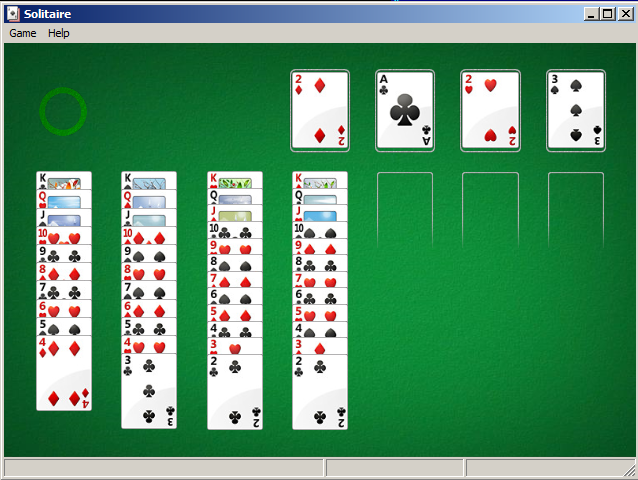
\includegraphics[width=0.6\textwidth]{examples/lines/1.png}
\caption{This is how the game is usually looks like}
\label{fig:lines_1}
\end{figure}

\clearpage
\myindex{\CStandardLibrary!rand()}

So let's see, is it be possible to find the random generator and do some trick with it.
\IDA quickly recognize the standard \TT{\_rand} function in \TT{balltrix.exe} at \TT{0x00403DA0}.
\IDA also shows that it is called only from one place:

\lstinputlisting[style=customasmx86]{examples/lines/random.lst}

We'll call it \q{random}.
Let's not to dive into this function's code yet.

This function is referred from 3 places.

Here are the first two:

\lstinputlisting[style=customasmx86]{examples/lines/1.lst}

Here is the third one:

\lstinputlisting[style=customasmx86]{examples/lines/2.lst}

So the function has only one argument.

10 is passed in first two cases and 5 in third.
We can also notice 
that the board has a size of 10*10 and there are 5 possible colors.
This is it!
The standard \TT{rand()} function returns 
a number in the \TT{0..0x7FFF} range and this is often inconvenient,
so many programmers implement their own random functions which returns a random number in a specified range.
In our case, the range is $0..n-1$ and $n$ is passed as the sole argument of the function.
We can quickly check this in any debugger.

So let's fix the third function call to always return zero.
First, we will replace three instructions (\TT{PUSH/CALL/ADD}) 
by \ac{NOP}s.
Then we'll add \INS{XOR EAX, EAX} instruction, 
to clear the \EAX register.

\lstinputlisting[style=customasmx86]{examples/lines/fixed.lst}

So what we did is we replaced a call to the \TT{random()} 
function by a code which always returns zero.

\clearpage
Let's run it now:

\begin{figure}[H]
\centering
\includegraphics[width=0.6\textwidth]{examples/lines/2.png}
\caption{Practical joke works}
\end{figure}

Oh yes, it works\footnote{Author of this book once did this as a joke for his coworkers with 
the hope that they would stop playing. They didn't.}.

But why are the arguments to the \TT{random()} functions global variables?
That's just because it's possible to change the board size in the game's settings, 
so these values are not hardcoded.
The 10 and 5 values are just defaults.
